\documentclass[12pt]{article}

\usepackage[french]{babel}
\usepackage[utf8x]{inputenc}
\usepackage[T1]{fontenc}
\usepackage{float}
\usepackage{amsmath}
\usepackage{graphicx}
\usepackage{url}
\usepackage[pdfborder={0 0 0}]{hyperref}
\usepackage{array}
\usepackage{tabularx}
\usepackage{setspace}
\usepackage{abstract}
\usepackage[top=2cm, bottom=2cm, left=2cm, right=2cm]{geometry}
\usepackage{subfig}
\usepackage{tabulary}
\usepackage{xcolor}
\usepackage{listings}
\lstset{basicstyle=\ttfamily\color{darkgray},
		numbers=left,
		frame=single,
		breaklines=true,
		stringstyle=\color{PineGreen},
		commentstyle=\color{Tan},
		extendedchars=true,
		keywordstyle=\bfseries\color{RedOrange}}

% A rajouter si on veut ajouter les paragraphes et subparagraphes à la TOC
%\setcounter{secnumdepth}{4}
%\setcounter{tocdepth}{4}


\begin{document}

% Le fichier plein de bordel pour la page de garde et le titre...
\newcommand{\HRule}{\rule{\linewidth}{0.5mm}}


\begin{titlepage}
\begin{center}


\includegraphics[width=0.35\textwidth]{img/Logo-groupe.png}
\hspace{5cm}

\includegraphics[width=0.35\textwidth]{img/Logo-telecom.png}~\\[1cm]
\vspace{1cm}


\textsc{\Large }\\[0.5cm]

\HRule \\[0.4cm]

{\huge \bfseries
Installation et supervision d'une architecture d'annuaire \\[0.4cm] }

\HRule \\[2cm]

\includegraphics[width=0.25\textwidth]{img/logo_exia.jpg}~\\[1cm]
\textsc{\LARGE eXia.CESI Lyon}\\[1.5cm]

\vspace{2.5cm}

\begin{minipage}{0.5\textwidth}
\begin{flushleft} \large
\emph{Auteurs:}\\
BLOCHET \textsc{Tanguy}\\
SACLIER \textsc{Baptiste}\\
PONSARD \textsc{Jean-Guillaume}
\end{flushleft}
\end{minipage}
\begin{minipage}{0.4\textwidth}
\begin{flushright} \large
\emph{Client:} \\
iSEC \textsc{GROUP}
\end{flushright}
\end{minipage}

\vfill

{\large \today}

\end{center}
\end{titlepage}

\newpage
~
\thispagestyle{empty}
\newpage

\tableofcontents
\thispagestyle{empty}
\setcounter{page}{0}

\renewcommand{\arraystretch}{1.5}

~
\thispagestyle{empty}
\setcounter{page}{0}
\newpage

% Partie pour la présentation du sujet et du besoin
\section{Situation}
	\paragraph{}
		Ce projet avait pour but de nous faire réaliser une architecture d'annuaire en installant des services qui reposent sur l'Active Directory et la supervision de serveurs. L'architecture a réaliser est pour le compte du groupe iSEC dont l'organisation est schématisé dans la figure \ref{isec_orga}.

		\begin{figure}[h]
			\centering
			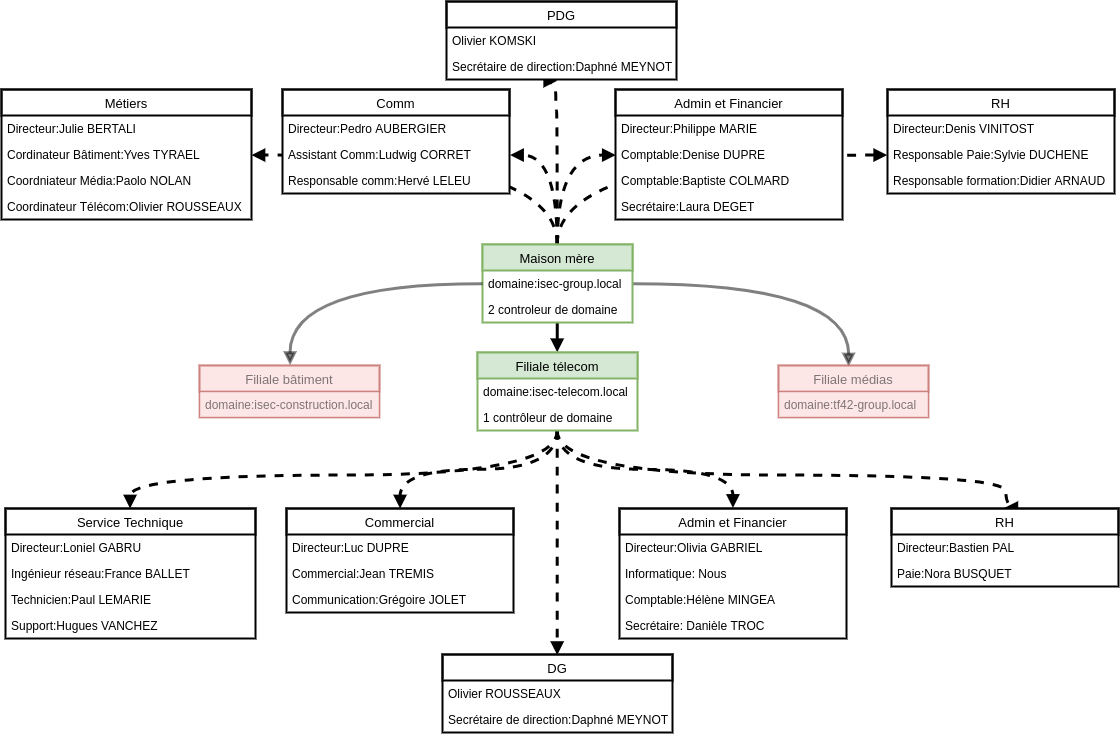
\includegraphics[scale=0.45]{Presentation/img/ISEC_orga.png}
			\caption{Schéma de l'organisation de groupe iSEC.}
			\label{isec_orga}
		\end{figure}
	\paragraph{}
		Le groupe iSEC, qui vient de racheter une entreprise, est présent dans plusieurs secteurs d'activités et possède donc plusieurs filiales. Il souhaite connecter le réseau de la maison mère avec celle des filiales. Notre but est de mettre en \oe{}uvre l'architecture Active Directory de la maison mère et de la filiale télécom uniquement.
	\subsection{Besoins techniques}
		\paragraph{}
			Les besoins techniques sont nombreux, mais le principal est de relier la maison mère et la filiale télécom avec un Active Directory. Le groupe iSEC doit avoir un contrôleur de domaine principal ainsi qu'un réplica pour la continuité de service. Le groupe télécom lui doit avoir un seul contrôleur de domaine. De plus une \textbf{relation d'approbation unidirectionnelle} entre les deux fôrets doit être mise en place, les utilisateurs du domaine groupe peuvent accéder aux ressources du domaine de la filiale télécom mais pas l'inverse.
		\paragraph{}	
			L'arborescence de l'Active Directory doit être créée et organisée selon les organigrammes du groupe et de sa filiale. De nombreux partages doivent ensuite être disponibles entre services, groupes et utilisateurs. D'autres service doivent être proposés par l'Active Directory comme l'installation automatique de 7Zip, la mise en place de fond d'écran et bien d'autre services qui sont décris dans les procédures d'installation qui suivent.
	\subsection{Organisation}
		\paragraph{}
			Ce projet a commencé le lundi 4 décembre et se termine le mardi 12 novembre. Les taches ont été découpées comme dans la figure \ref{planning} :

			\begin{figure}[h]
				\centering
				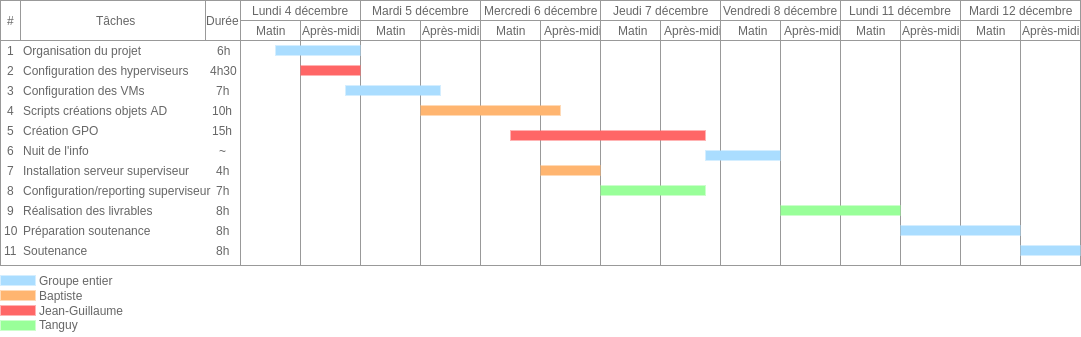
\includegraphics[scale=0.50]{Presentation/img/Planning_previsio.png}
				\caption{Planning prévisionnel du projet.}
				\label{planning}
			\end{figure} 

		\paragraph{}
			Ce planning prévisionnel a été dans l'ensemble respecté, certaines heures supplémentaires ont été nécessaires pour la configuration des serveurs de supervision. Un dépot Github a été créé afin de conserver les différents scripts utilisés pendant ce projet ainsi que les sources de ce rapport, il est disponible à ce lien : \href{https://github.com/Exia-epickiwi/Projet-iSEC}{https://github.com/Exia-epickiwi/Projet-iSEC}

% Partie pour les procédures d'installation des serveurs
\section{Installation des serveurs}
	\subsection{Hyperviseur}
		% Décrire le choix d'hyperviseur et sa configuration si besoin

	\subsection{Machines virtuelles}
		% Décrire installation des machines virtuelles

	\subsection{Communication inter-VMs}
		% Décrire notre architecture pour communiquer, commutateur, NAT, routeur...

% Partie pour la configuration des serveurs
\section{Configuration des serveurs}

Afin de configurer un domaine Active Directory au sein d’un réseau Windows sur un serveur Windows Server 2012 R2, il faut suivre les étapes suivantes :
L’installation de fonctionnalités sous Windows Server se fait par l’installation de rôles : dans le tableau de bord du gestionnaire de serveur Windows Server 2012, il faut cliquer sur « Gérer » puis « Ajoutez des rôles et fonctionnalités ». Ensuite, il faut cliquer sur « Suivant » puis sélectionner « Installation basée sur un rôle ou une fonctionnalité », ensuite il faut sélectionner le « Pool de serveur » (nous sélectionnons notre serveur) puis cliquer sur « Suivant ». Il est alors possible de sélectionner les rôles à installer.


	\subsection{Serveurs groupe iSEC}	
		\subsubsection{Serveur principal}
-	Installer le rôle AD DS :
Ce rôle permet d’installer l’Active Directory : Annuaire Microsoft permettant de regrouper toutes les informations du réseau. 
Dans la fenêtre de sélection des rôles, Sélectionner le rôle AD DS. Le fait de sélectionner ce rôle installe automatiquement le rôle DNS (indispensable pour le bon fonctionnement de l’Active Directory).
Ensuite, il faut valider jusqu’à l’installation et cliquer sur « Installer ». Il est recommandé d’attribuer une adresse IP fixe au serveur avant d’installer le rôle. De plus ceci sera utile par la suite pour configurer le DHCP.

-	Configurer le rôle AD DS :
Une fois le rôle installé, dans le tableau de bord du gestionnaire de serveur, il faut cliquer sur « Promouvoir le serveur en tant que contrôleur de domaine ». Une fenêtre s’ouvre et demande les actions à effectuer. Il faut Sélectionner « Ajouter une nouvelle forêt » et entre le nom de celle-ci : « isec-group.local » puis cliquer sur « Suivant ». Ensuite, il faut renseigner un mot de passe du mode de restauration des services d’annuaire et cliquer sur « Suivant » puis « Suivant » jusqu’à arriver à l’installation. Ensuite, cliquer sur « Installer ». Le serveur redémarrera automatiquement à la fin de cette opération. L’Active Directory est désormais fonctionnel.

-	Installer le rôle DHCP :
Vous devez attribuer une adresse IP statique au serveur avant d’installer le DHCP.
Ensuite, il faut sélectionner « Serveur DHCP » dans le menu d’installation des rôles et fonctionnalités et cliquer sur « Suivant » jusqu’à arriver au menu d’installation où il faut cliquer sur « Installer ». Avant de cliquer sur « Fermer », il faut cliquer sur « Terminer la configuration DHCP » et valider les deux étapes.

-	Configurer le DHCP :
Une fois l’installation terminée, il faut ouvrir le gestionnaire DHCP qui se trouve dans l’onglet « Outils » du gestionnaire de serveur. Il faut faire un clic droit sur IPv4 et ouvrir « nouvelle étendue ». Un assistant de création de la nouvelle étendue s’affiche. Il demande de nommer l’étendue (vous pouvez mettre le nom de votre choix) et de mettre une description (facultative). 
Ensuite, il faut rentrer l’adresse IP de début et de fin de la plage d’adressage disponible pour les ordinateurs de l’AD. La section « Paramètres de configuration qui se propagent au client DHCP » se rempli automatiquement. Il est ensuite possible d’exclure une plage d’adresse IP si nécessaire. Ensuite, il faut définir la durée du bail des adresses. Ensuite, il est demandé d’indiquer la passerelle par défaut (routeur du réseau), puis le serveur DNS (les options sont automatiquement remplies car le DNS est sur le serveur en question). Il suffit ensuite de cliquer sur « Suivant » jusqu’à arriver à la fin de l’assistant. 
Le serveur DHCP est maintenant fonctionnel.

		\subsubsection{Serveur réplica}
L’installation du rôle s’effectue de la même manière que pour le serveur ISEC-GROUP-MASTER. Seule la configuration diffère : Lors de la promotion du serveur en tant que contrôleur de domaine, il faut sélectionner « Ajouter ce contrôleur de domaine à un domaine existant » et spécifier le domaine en question. Il faut ensuite entrer le mot de passe DSRM puis cliquer sur « Suivant ». Ensuite, il faut vérifier que le serveur ISEC-GROUP-MASTER soit sélectionné en tant que source de réplication puis cliquer sur « Suivant » jusqu’à arriver à l’installation. Une fois le redémarrage terminé, le réplica est fonctionnel et il est possible d’accéder aux informations de l’Active Directory.
	\subsection{Serveurs groupe Telecom}
		\subsubsection{Serveur Windows Server}
L’installation et la configuration de ce serveur est quasi identique à celle de ISEC-GROUP-MASTER à l’exception que le nom de domaine est différent. Il ne faut également pas installer de DHCP car ISEC-GROUP-MASTER dispose déjà d’un DHCP.

% Partie pour la réponse technique au besoin
% Pas trop d'idée pour ce nom de section à revoir...
\section{Réponse au besoin}
	\subsection{Scripts}
	\subsection{GPO}
		\subsubsection{Partage Groupe}
		\subsubsection{Partage Telecom}
		\subsubsection{Partage par service}
		\subsubsection{Imprimantes}
		\subsubsection{Sécurité mot de passe}
		\subsubsection{Exécution automatique}
		\subsubsection{Fond d'écran}
		\subsubsection{Logiciel 7Zip}
		\subsubsection{...}

% Partie pour la supervision des serveurs
\section{Supervision}
	\subsection{Installation}
	\subsection{Configuration}
	

% Partie pour le bilan de ce rapport
\section{Bilan}
	\subsection{Évolutions possibles}
		\paragraph{}
			Les différentes GPOs créées pourraient être déployés avec des scripts powershell afin de recréer les GPO d'un domaine sur un deuxième domaine. De nombreuses autres GPOs pourraient être mises en place, que ce soit au niveau de la sécurité, que de la personnalisation du poste utilisateur.
	\subsection{Conclusion}
		\subsubsection{Tanguy Blochet}
			\paragraph{}
				Ce projet a été très intéressant, il m'a permis de mettre en application toutes les connaissances étudiées en prosit. Il a fallu beaucoup de patience pour ce projet, que ce soit pour l'installation, ou le redémarrage des machines virtuelles. Le groupe a eu une très bonne entente et a très bien fonctionné.
		\subsubsection{Baptiste Saclier}
			\paragraph{}

		\subsubsection{Jean-Guillaume Ponsard}	
			\paragraph{}



\newpage


\end{document}
